\documentclass[conference]{IEEEtran}

\usepackage{cite}
\usepackage{amsmath,amssymb,amsfonts}
\usepackage{algorithmic}
\usepackage{graphicx}
\usepackage{subcaption}
\usepackage{textcomp}
\usepackage{xcolor}
\usepackage{subfigure}
\usepackage{amsfonts}
\usepackage{booktabs}
\usepackage{multirow}
\usepackage{hyperref}

\begin{document}

\title{CS 352 - Introduction to Reinforcement Learning \\ Habib University \\ {\large Project Report, Spring 2023} \\ {\LARGE Impact of $\alpha$ in Q-Learning}}


\author{\IEEEauthorblockN{Mohammed Haider Abbas}
\IEEEauthorblockA{\textit{Dhanani School of Science and Engineering} \\
\textit{Habib University}\\
ma06418@st.habib.edu.pk}
\and
\IEEEauthorblockN{Muhammad Ahsan}
\IEEEauthorblockA{\textit{Dhanani School of Science and Engineering} \\
\textit{Habib University}\\
ma06371@st.habib.edu.pk}
}

\maketitle

\begin{abstract}
 In this research paper, we focus on the impact of the learning rate parameter, $\alpha$, on the performance of Q-learning. We compare the performance of Q-learning for various values of $\alpha$. Specifically, we evaluate the impact of $\alpha$ on two key performance metrics: computational efficiency, i.e., the time taken to converge, and maximizing reward, i.e., the average reward obtained by running the learned policies for various starting states. We have implemented the Q-learning algorithm on the Taxi learning problem using OpenAI's Gym Toy Text Taxi environment. The $\alpha$ value that results in the highest average reward should be identified to determine which $\alpha$ value is more effective at maximizing reward. 
 \newline
\end{abstract}
\section{Introduction}
Reinforcement learning is a subfield of machine learning that involves learning through interaction with an environment. The goal is for an agent to learn optimal behavior in the environment through trial and error. The Q-learning algorithm is one of the most popular reinforcement learning algorithms and has been successfully applied to a variety of problems. \\ \\ Q-learning \cite{1} is a model-free, off-policy algorithm that seeks to learn the optimal action-value function for a given task. The algorithm iteratively updates the Q-values of each state-action pair based on the rewards received by the agent and the predicted future rewards. By iteratively improving the policy based on the learned Q-values, the agent can eventually converge to an optimal policy that maximizes the expected cumulative reward over time. \\ \\ The Taxi Problem\cite{2} is a classical problem in Reinforcement Learning. In this problem, the agent (taxi) needs to pick up the passenger from one of the four colored place and deliver the passenger to the destination (also one of the four colored place). The game is in 5 by 5 grid world. There are six actions that are available to the agent in this game: LEFT, RIGHT, UP, DOWN, PICKUP and PUTDOWN. The first four action will make the agent move 1 step forward according to the direction of the action, but won't have effect when the agent hits the wall or boundaries. At each step, the agent will receive a reward of -1. However, when the delivery is achieved, it will receive a reward of 20. In some conditions, several actions are illegal. This includes but not limited to take PUTDOWN action when there is no passenger in the taxi or it is not the destination spot, PICKUP a passenger where there is no passenger and so on. All these illegal action will cause a reward of -10 and change nothing. Thus, without any state abstraction, there are totally 500 states, including 25 position of the taxi, 4 possible location of the destination, and 5 possible location of the passenger (four colors and taxi). \\ \\ In this paper, we investigate the performance of $\alpha$ in Q-learning algorithm on the Taxi-v3 environment \cite{3} which is a part of OpenAI's GYM Toy Text framework. The remainder of this paper is organized as follows. In Section 2, we describe the problem formulation and the methodology used in our experiments. Section 3 presents and discusses the experimental results, and Section 4 concludes the paper by summarizing the main findings and their implications.

\section{Methodology}
The source code for our Q-learning implementation can be found at the following Github repository: \href{https://github.com/haider-06418/RL-Project/tree/main}{Project Repository}. The experiments were conducted using the default hyperparameters, with the exception of the learning rate parameter $\alpha$, which was varied across a range of values access the algorithm in terms of computational efficiency and maximizing reward.

\subsection{Setup:}
All experiments were conducted using Python 3.10 in the VS Code development environment. The following are the main Python libraries used:
\begin{itemize}
\item OpenAI Gym
\item NumPy
\item Matplotlib
\end{itemize}

\subsection{Problem Formulation:}
We consider the Taxi-v3 environment from the OpenAI Gym as our testbed. The objective of the environment is for the agent, a taxi, to navigate through a grid-world to pick up and drop off passengers at specified locations. The state space of the environment is discrete, and the action space is finite.
\newline
\subsubsection{Description} 
There are four designated locations in the grid world indicated by R(ed), G(reen), Y(ellow), and B(lue). When the episode starts, the taxi starts off at a random square and the passenger is at a random location. The taxi drives to the passenger's location, picks up the passenger, drives to the passenger's destination (another one of the four specified locations), and then drops off the passenger. Once the passenger is dropped off, the episode ends.
\newline
\subsubsection{Actions}
There are 6 discrete deterministic actions:
\begin{itemize}
    \item move south
    \item move north
    \item move east
    \item move west
    \item pickup passenger
    \item drop off passenger
    \newline
\end{itemize}
\subsubsection{Grid World}
There are 500 discrete states since there are 25 taxi positions, 5 possible locations of the passenger (Red, Green, Yellow, Blue, in Taxi), and 4 destination locations (Red, Green, Yellow, Blue). Note that there are 400 states that can actually be reached during an episode. The missing states correspond to situations in which the passenger is at the same location as their destination, as this typically signals the end of an episode. Four additional states can be observed right after a successful episodes, when both the passenger and the taxi are at the destination. This gives a total of 404 reachable discrete states. Each state space is represented by the tuple: (taxi\_row, taxi\_col, passenger\_location, destination). An observation is an integer that encodes the corresponding state. The state tuple can then be decoded with the "decode" method.
\newline
\subsubsection{Rewards}
Rewards are as follows:
\begin{itemize}
    \item -1 per step unless other reward is triggered.
    \item +20 delivering passenger.
    \item -10  executing "pickup" and "drop-off" actions illegally.
    \newline
\end{itemize}

\subsection{Algorithm Implementation:}
We implemented Q-learning in Python using the OpenAI Gym toolkit. We have used the tabular Q-learning approach \cite{4}, which maintains a table of state-action values, to learn the optimal policy. We initialize the Q-values to 0 for all state-action pairs and use a decayed epsilon-greedy policy to explore the state space. 

\subsection{Hyperparameters:}
\subsubsection{$\alpha$}
The range for $\alpha$ is 0 $\leq \alpha \leq$ 1. We vary the learning rate, alpha - $\alpha$, from 0.1 to 0.9 in increments of 0.1 and evaluate the performance of the algorithm for each $\alpha$ value. For investigating corner cases we also have tested for $\alpha$ from 0 to 1 in increments of 0.1 to get to know of its behaviour on 0 and 1. In addition to the aforementioned $\alpha$ values, we also tested for very small and very large $\alpha$ values. Very small $\alpha$ values ranged from 0.01 to 0.09 in increments of 0.01 and very large $\alpha$ values were from 0.90 to 0.99 in increments of 0.01. 
\newline
\subsubsection{Other hyperparameters}
We do not tune any other hyperparameters, such as the discount factor, epsilon decay rate, and the number of episodes, to ensure that the impact of $\alpha$ is fairly compared. The hyperparameters set throughout are as follows: 
\begin{itemize}
    \item Discount rate - $\gamma$ = 1.0
    \item Exploration rate - $\epsilon$ = 0.1
    \item Number of episodes = 10000
    \newline
\end{itemize} 

\subsection{Performance Metrics:}
We evaluate the performance of the Q-Learning algorithm in terms of two metrics: computational efficiency, i.e., the time taken to converge, and maximizing reward, i.e., the average reward obtained by running the learned policies for various starting states. To measure computational efficiency, we record the average running time required for the algorithm to converge to an optimal policy. To measure maximizing reward, we run the learned policies for each $\alpha$ value for various starting states and calculate the average reward. 

\subsection{Experimental Setup:}
We conduct a total of 5 independent runs for each $\alpha$ value and take the mean of both the performance metrics; time taken to converge and reward. We use various starting states assigned randomly for each experiment and randomize the location of the passenger and destination in each episode to ensure that the our Q-learning algorithm generalize to different scenarios. 

\section{Results}
Our results showed that the choice of $\alpha$ had a significant impact on the agent's performance. Choosing an appropriate value for $\alpha$ is important for the Q-learning algorithm to converge to the optimal policy. \\ \\ Our results, Plots 1 and 2 shown below (each plot is an independent run) show that if $\alpha$ is too high, the agent may overreact to new information hence may require more time to converge in turn lowering reward. Similarly if $\alpha$ is too low, the agent may be slow to learn hence may require more time to converge or fail to converge in turn lowering reward. As evident through as results below, the learning rate at which we are getting the maximum reward is in the range of 0.4 to 0.6, mostly at 0.5, and at this range the agent is taking the least time to converge. Therefore, the learning rate should be set some where in between 0.4 and 0.6 as we saw that we are getting maximum reward. 
% plot 2 and 5
\begin{figure*}[htbp]
    \centering
    \begin{minipage}[b]{0.45\linewidth}
        \centering
        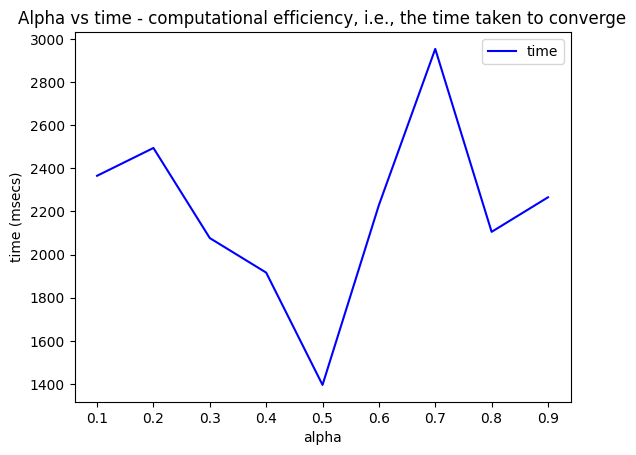
\includegraphics[width=\textwidth]{Plots/alpha vs time 2.png}
        \caption{Plot 1 - Alpha vs Time}
        \label{fig:figure1}
    \end{minipage}
    \hfill
    \begin{minipage}[b]{0.45\linewidth}
        \centering
        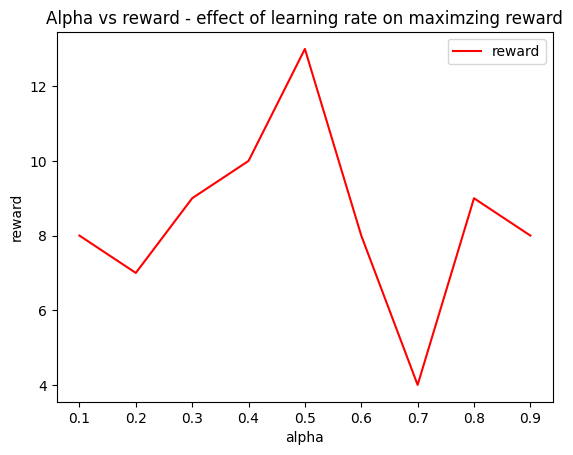
\includegraphics[width=\textwidth]{Plots/alpha vs reward 2.png}
        \caption{Plot 1 - Alpha vs Reward}
        \label{fig:figure2}
    \end{minipage}

    \vspace{0.5cm}

    \begin{minipage}[b]{0.45\linewidth}
        \centering
        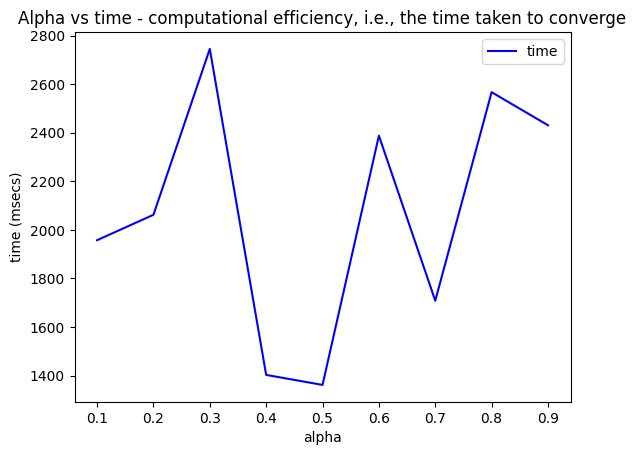
\includegraphics[width=\textwidth]{Plots/alpha vs time 5.png}
        \caption{Plot 2 - Alpha vs Time}
        \label{fig:figure3}
    \end{minipage}
    \hfill
    \begin{minipage}[b]{0.45\linewidth}
        \centering
        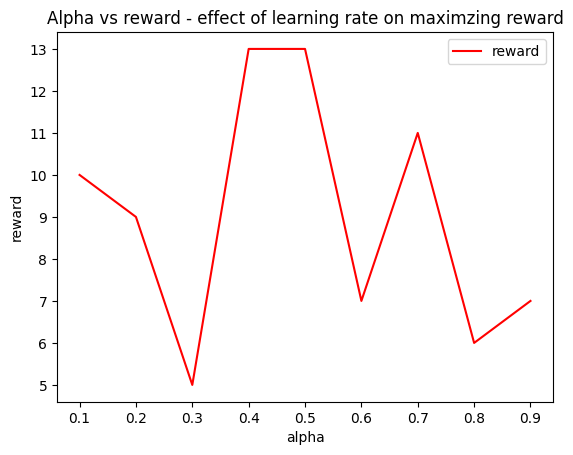
\includegraphics[width=\textwidth]{Plots/alpha vs reward 5.png}
        \caption{Plot 2 - Alpha vs Reward}
        \label{fig:figure4}
    \end{minipage}
\end{figure*}

For cases such as very low or very high $\alpha$ values, the time taken to converge was higher than normal range of $\alpha$ values such as seen below in plot 3 of very small $\alpha$ values ranged from 0.01 to 0.09 in increments of 0.01. Here we can also notice that as we approach to 0.09, we are maximizing reward and getting less time to converge. This supports our stance that for very small $\alpha$ values, the agent will not maximize reward and will take longer to converge but as 0.09 is close to 0.1 which is relatively a larger value than all of the $\alpha$ values in the range therefore it will maximize reward and take least time to converge. 
% plot cc 1 
\begin{figure}[htbp]
  \centering
  \begin{subfigure}[t]{0.45\linewidth}
    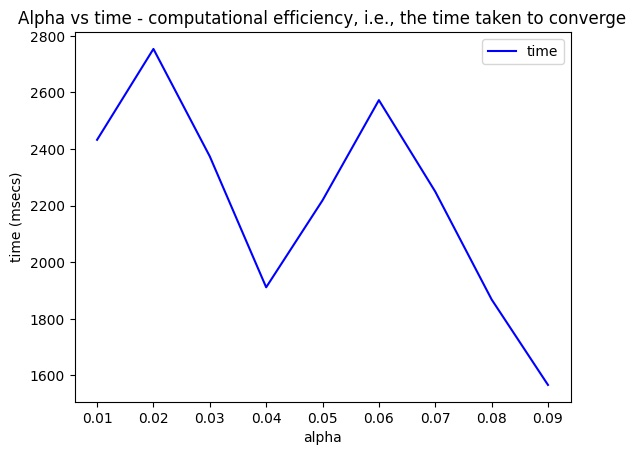
\includegraphics[width=\linewidth]{Plots/alpha vs time cc 1.jpg}
    \caption{Alpha vs Time}
    \label{fig:figure98}
  \end{subfigure}
  \hfill
  \begin{subfigure}[t]{0.45\linewidth}
    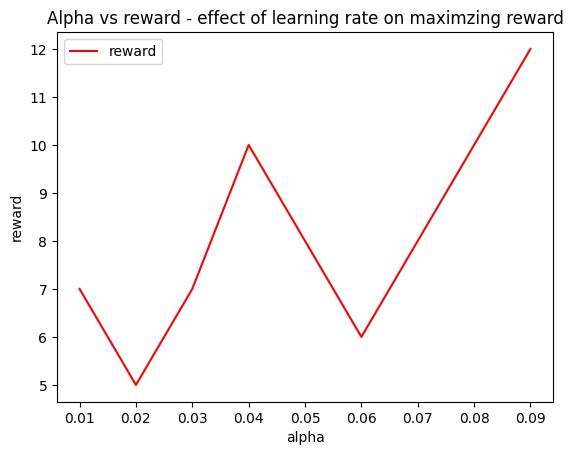
\includegraphics[width=\linewidth]{Plots/alpha vs reward cc 1.jpg}
    \caption{Alpha vs Reward}
    \label{fig:figure99}
  \end{subfigure}
  \caption{Plot 3}
  \label{fig:bothfigures}
\end{figure}
\newline
\begin{figure}[htbp]
  \centering
  \begin{subfigure}[t]{0.45\linewidth}
    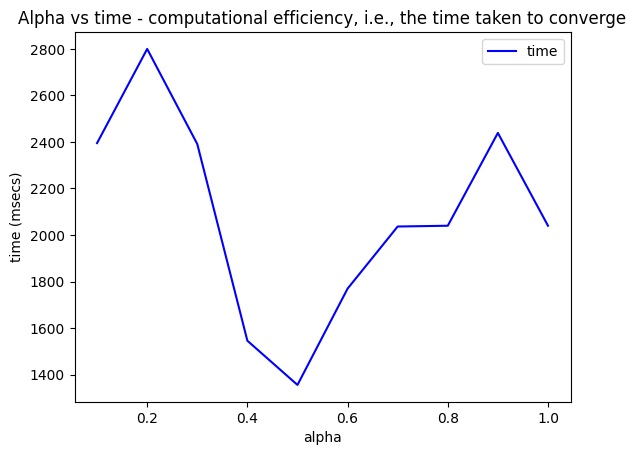
\includegraphics[width=\linewidth]{Plots/alpha vs time 6.jpg}
    \caption{Alpha vs Time}
    \label{fig:figure90}
  \end{subfigure}
  \hfill
  \begin{subfigure}[t]{0.45\linewidth}
    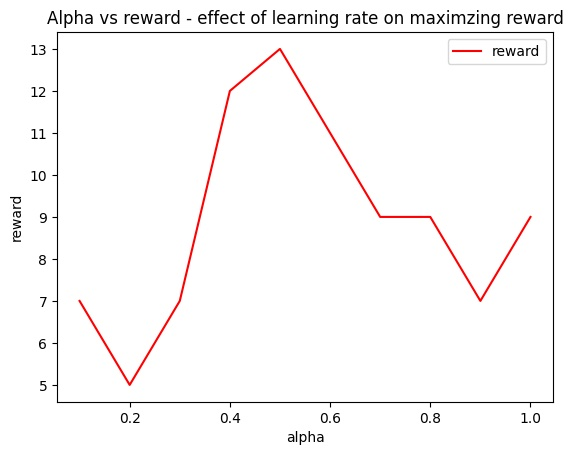
\includegraphics[width=\linewidth]{Plots/alpha vs reward 6.jpg}
    \caption{Alpha vs Reward}
    \label{fig:figure91}
  \end{subfigure}
  \caption{Plot 4}
  \label{fig:bothfigures}
\end{figure}

For $\alpha$ equal to 0, our agent was failing to converge since the program kept running which tells it did not converge. All runs for $\alpha$ = 0 were aborted after running for 5 minutes since it was not converging. For $\alpha$ equal to 1 our test went as expected and it took more time to converge and did not maximize reward, as shown by plot 4. Plot 4 in addition to plots 1 and 2 also highlights our finding that at 0.4 $ \leq \alpha \leq$ 0.6 we are getting maximum reward and least time to converge. Exact $\alpha$ at which we are getting maximum reward and least time to converge is $\alpha$ = 0.5 for plot 4 on next page. \\ \\ Our study also highlights the relation between time taken to converge and reward. After analyzing on the data for time vs reward, we can conclude that they have an inverse relation, i.e. for a Q-Learning Problem, the time taken to converge is inversely proportional to the reward obtained or in other words maximizing reward is inversely proportional to computational efficiency i.e. time taken to converge. All the above result plots also prove this that an agent takes less time to obtain maximum reward and vice versa. The following plots (all independent and separate runs) also back our findings as it can be seen that for more time the reward is less and for less time the reward is more. 

\begin{figure}[htbp]
  \centering
  \begin{subfigure}[t]{0.45\linewidth}
    \centering
    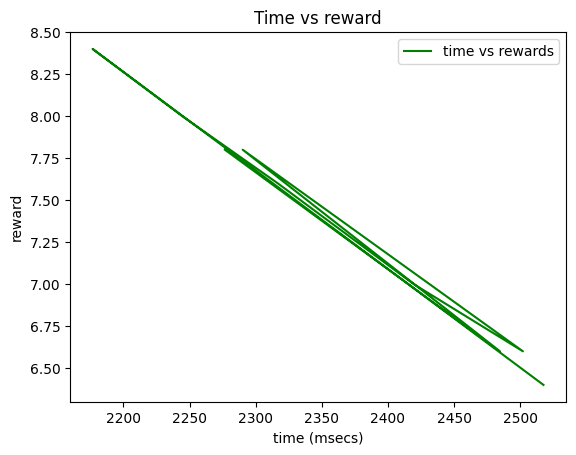
\includegraphics[width=\linewidth]{Plots/tvr 1.png}
    \caption{Plot 5 - Time vs Reward}
    \label{fig:figure89}
  \end{subfigure}
  \hfill
  \begin{subfigure}[t]{0.45\linewidth}
    \centering
    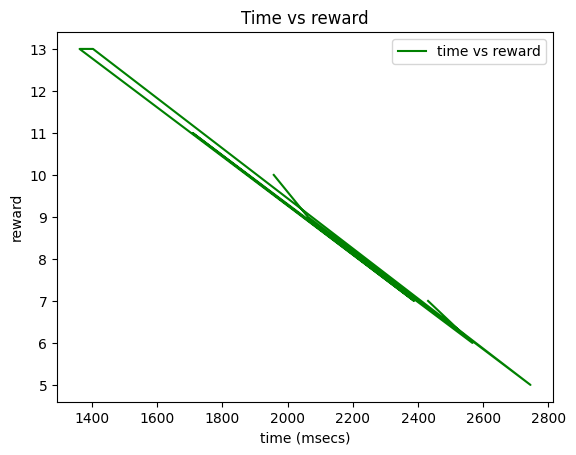
\includegraphics[width=\linewidth]{Plots/trv2.png}
    \caption{Plot 6 - Time vs Reward}
    \label{fig:figure88}
  \end{subfigure}
  
  \vspace{0.5cm}
  
  \begin{subfigure}[t]{0.45\linewidth}
    \centering
    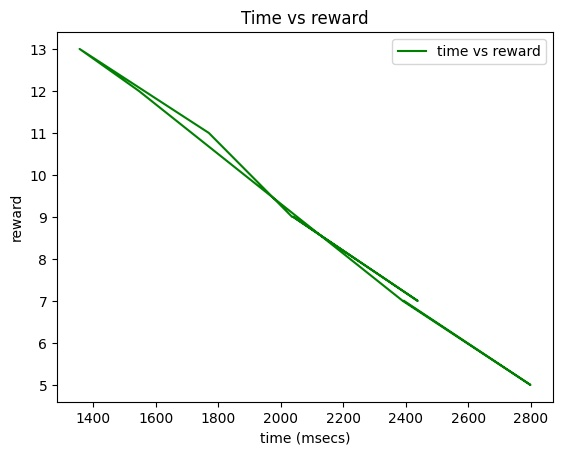
\includegraphics[width=\linewidth]{Plots/tvr 3.jpg}
    \caption{Plot 7 - Time vs Reward}
    \label{fig:figure87}
  \end{subfigure}
  \hfill
  \begin{subfigure}[t]{0.45\linewidth}
    \centering
    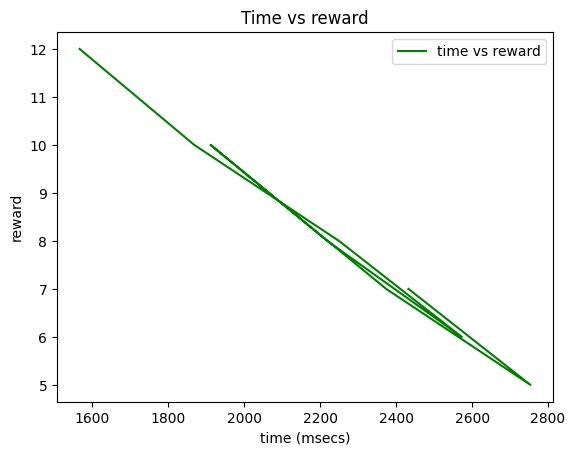
\includegraphics[width=\linewidth]{Plots/tvr cc 1.jpg}
    \caption{Plot 8 - Time vs Reward}
    \label{fig:figure86}
  \end{subfigure}
  \caption{Plot 5 - 8: Time vs Reward Plots}
  \label{fig:allfigures}
\end{figure}
 
\section{Conclusion}
 In this study, we analyzed the performance of Q-learning algorithm for various values of the learning rate parameter, $\alpha$. We evaluated the performance of the agent in terms of computational efficiency and the ability to maximize rewards. \\ \\ Our results and findings can be summarized such that the choice of $\alpha$ has a significant impact on the performance of the agent. The range for $\alpha$ is 0 $\leq \alpha \leq$ 1. For low and high values of $\alpha$, the agent did not maximize reward and was taking more time to converge. For low values of $\alpha$ the agent was slow to learn hence requiring more time to converge (or failed to converge at 0) and for high values of $\alpha$ the agent was overreacting to new information hence requiring more time to converge. Therefore the optimal range of $\alpha$ where it gave maximum reward and was computationally efficient i.e. faster convergence was in the range of 0.4  $\leq \alpha \leq$ 0.6 with the most optimal value of $\alpha$ being at 0.5. Our findings also led to discovering the relationship between converge time and reward, such that maximizing reward is inversely proportional to computational efficiency i.e. time taken to converge. More the time taken to converge, less the reward and vice verse. \\ \\ In conclusion, this study highlights the importance of selecting an appropriate learning rate parameter for Q-learning algorithm in reinforcement learning. By selecting an appropriate $\alpha$ value within a certain range, we can optimize the performance of the Q-Learning algorithm. 

\section*{Acknowledgment}
We would like to thank Brendon Martin and Satwick Kansal for their guide \cite{5} on solving the Taxi problem with Q-learning. 

\begin{thebibliography}{00}
\bibitem{1} P. Labarta Bajo, “Reinforcement Learning [Part 2]: The Q-learning Algorithm | HackerNoon,” hackernoon.com, Mar. 28, 2022. https://hackernoon.com/reinforcement-learning-part-2-the-q-learning-algorithm (accessed May 06, 2023).
\bibitem{2} G. Mayers, “Reinforcement Learning: Using Q-Learning to Drive a Taxi!,” Medium, Jul. 30, 2020. https://medium.com/analytics-vidhya/reinforcement-learning-using-q-learning-to-drive-a-taxi-5720f7cf38df (accessed May 05, 2023).
‌\bibitem{3} “Taxi - Gym Documentation,” www.gymlibrary.dev. https://www.gymlibrary.dev/environments/toy\_text/taxi/
\bibitem{4} C. De-Yu, “Q-Learning and SASAR, with Python,” Medium, Jul. 09, 2021. https://towardsdatascience.com/q-learning-and-sasar-with-python-3775f86bd178 (accessed May 05, 2023).
‌\bibitem{5} B. Martin and S. Kansal, “Reinforcement Q-Learning from Scratch in Python with OpenAI Gym,” Learndatasci.com, 2019. https://www.learndatasci.com/tutorials/reinforcement-q-learning-scratch-python-openai-gym/ (accessed May 03, 2023).
‌
\end{thebibliography}


\end{document}
